% \begin{document}
\chapter{Problemi e Modelli}

\section{Problemi di ottimizzazione}

\dfn{Ricerca operativa}{
  La \textbf{ricerca operativa} è un ramo della matematica applicata che si occupa dello studio, della modellizzazione e della risoluzione dei cosiddetti \textit{problemi decisionali} complessi mediante strumenti matematici, algoritmici e computazionali, con l'obiettivo di ottimizzare processi e risorse
}

Per evitare qualsivoglia fraintendimento fornirò anche la definizione di \textbf{ottimizzazione Combinatoria}
\dfn{Ottimizzazione Combinatoria}{
  Si definisce \textbf{Ottimizzazione Combinatoria} una branca della Ricerca Operativa che nel modellare matematicamente e risolvere problemi complessi di natura discreta unisce tecniche di calcolo combinatorio alla teoria degli algoritmi e ai risultati teorici e metodologici della programmazione lineare
}

Pertanto ricerca operativa e ottimizzazione combinatoria sono due cose diverse, MA cito testualmente
\begin{quote}
  "Per tutti i nostri scopi ricerca operativa e ottimizzazione, sono sinonimi

  tuttavia non vedremo solo alcune tecniche di ottimizzazione combinatoria, ma anche altre tecniche che stanno nella ricerca operativa ma che trattano di valori non discreti"

  \hfill -- Ugo
\end{quote}

Adesso, sotterrato questo problema di carattere unicamente terminologico con cui io non posso fare a meno di strizzarmi il cervello perché c'ho l'autismo, possiamo tornare a parlare di ricerca operativa/ottimizzazione combinatoria (tanto so' sinonimi per noi)

I problemi di cui si occupa la ricerca operativa, quindi, riguardano situazioni in cui occorra massimizzare i ricavi o minimizzare i costi, in presenza di risorse limitate. Detto in termini più matematici, data una funzione \textbf{vincolata} l'obiettivo è trovare una soluzione ottimale che massimizzi o minimizzi tale funzione.

È pertanto vero, quindi, che questa disciplina ha forte contenuto economico

La ricerca operativa si inserisce all'interno del processo decisionale, il quale può essere suddiviso in diverse fasi
\begin{itemize}
\item \textbf{Individuazione problema}
  \item \textbf{Raccolta dati}
    \item \textbf{Costruzione modello}, ovvero la Traduzione del problema in un modello matematico che descriva il sistema e i vincoli in modo formale
      \item \textbf{Determinazione di piu' soluzioni}: applicazione di algoritmi e tecniche di ottimizzazione per individuare la soluzione migliore 
  \item \textbf{Analisi dei risultati}
\end{itemize}

La ricerca operativa, quindi, si occupa delle fasi 3 e 4 del processo, dato che sono le fasi che richiedono l’impiego di modelli matematici, algoritmi di ottimizzazione e strumenti computazionali. Adesso andiamo a definire per benino che cosa intendiamo per "modello" 

\dfn{modello}{
  un \textbf{modello} è una descrizione astratta e scritta in linguaggio matematico, della parte di realtà utile al processo decisionale
}
I modelli ci permettono di inquadrare i problemi in una determinata "cornice" che ci permette di determinare quale tipo di algoritmo risolutivo usare.

Esistono tre tipi di modelli:
\begin{itemize}
\item \textbf{Teoria dei giochi}: ricerca di un equilibrio fra le componenti coinvolte in un'interazione reciproca, spesso con obbiettivi contrastanti. (non ce ne occupiamo)
\item \textbf{Simulazione}: il problema viene studiato simulando la situazione senza studiarne la natura in modo analitico tramite generazione di istanze casuali. (anche questi modelli non ci interessano)
\item \textbf{Analitici}: dal problema si costruisce un modello matematico rigoroso (senza perdere informazione sul problema reale) e risolto mediante tecniche analitiche, senza ricorrere a simulazioni. La natura stessa dello spazio matematico in cui è inserito il problema è in grado di garantire la soluzione ottima. Questo tipo approccio è particolarmente vantaggioso in quanto assicura l’esattezza della soluzione supponendo che il modello sia formulato correttamente. 

È tuttavia richiesto un discreto livello di creatività
\end{itemize}

Definiamo, adesso, i problemi che andiamo a trattare

\dfn{Problema}{
  Definiamo \textbf{problema} una domanda, espressa in termini generali, la cui risposta dipende da \textit{parametri} e \textit{variabili}, sopratutto nei problemi analitici
}
Un problema $ \mathcal{P} $ è descritto tramite:
\begin{itemize}
  \item I suoi parametri e variabili
  \item Le caratteristiche che una soluzione deve avere
\end{itemize}

Quando fissiamo un'istanza di un problema, vengono fissati i parametri ma non le variabili, che sono le incognite che devono essere definite. Distinguiamo un problema dalla sua istanza per generalizzarlo. Si presti attenzione alla differenza tra parametri e variabili che molti si confondono

\ex{Problema con paramteri e variabili}{
  Sia $ \mathcal{P} $ il seguente problema
  \[
    ax^2+bx+c =0
  \]
  Dove $a,b$ e $c$ sono i suoi parametri e $x$ rappresenta le variabili, una possibile istanza di tale problema è:
  \[
    5x^2-6x+1=0
  \] 
}
Un modo comune per descrivere un problema è dare l'insieme di soluzioni ammissibili $ \mathbb{F}_{\mathcal{P}} \subseteq G $, dove $G$ è un sovrainsieme generico noto, di solito contenente la collezione di tutte le possibili configurazioni o decisioni che si possono prendere, dando dei vincoli che un generico $ g \in G $ deve soddisfare per far parte di $\mathbb{F}_{\mathcal{P}}$, avremo così che $G - \mathbb{F}_{\mathcal{P}}$ è l'insieme delle soluzioni non ammissibili 
\ex{}{
  Sia l'instanza di $\mathcal{P}$ definita precedentemente
  \[
    5x^s - 6x+1= 0
  \]
  si ha che 
  \[
    \begin{array}{l}
      \mathbb{G}= \mathbb{R}\\
      \mathbb{F}_{\mathcal{P}} = \{x\in \mathbb{R} | 5x^2-6x+1=0\}
    \end{array}
  \]
}
\subsection{2.1.1 Problemi di ottimizzazione}

Iniziamo con una definizione preliminare.

\dfn{Problema di ottimizzazione}{In matematica e in informatica, un problema di ottimizzazione è il problema di trovare la migliore soluzione fra tutte le soluzioni fattibili.}

Un problema di ottimizzazione $\mathcal{P}$ viene descritto:
\begin{itemize}
  \item Dando l’insieme $\mathbb{F}_\mathcal{P}$ delle soluzioni ammissibili
  \item Specificando una funzione obiettivo $c_\mathcal{P} : \mathbb{F}_\mathcal{P} \to \mathbb{R}$ che assegna ad ogni $g \in \mathbb{F}_\mathcal{P}$ un valore reale $c_\mathcal{P}(g)$, che rappresenta il costo o il beneficio.
\end{itemize}
Un problema (di ottimizzazione) di massimo $\mathcal{P}$ consiste nel determinare il valore
\[
Z_\mathcal{P} = \max \{ c_\mathcal{P}(g) \mid g \in \mathbb{F}_\mathcal{P} \},
\]
mentre un problema (di ottimizzazione) di minimo $\mathcal{P}$ consiste nel determinare il valore
\[
Z_\mathcal{P} = \min \{ c_\mathcal{P}(g) \mid g \in \mathbb{F}_\mathcal{P} \}.
\]
Ci si può trastullare con la definizione, infatti ad ogni problema di massimo $\mathcal{P}$ corrisponde un problema di minimo $\mathcal{P}'$ tale che $c_{\mathcal{P}'}(g) = -c_\mathcal{P}(g)$, ovvero:
\[
Z_\mathcal{P} = -\min \{ c_{\mathcal{P}'}(g) \mid g \in \mathbb{F}_\mathcal{P} = \mathbb{F}_{\mathcal{P}'} \}.
\]

\dfn{Valore ottimo e soluzione ottima}{Dato un problema di ottimizzazione $\mathcal{P}$, il valore $Z_\mathcal{P}$ definito in precedenza è detto valore ottimo, mentre il $g^* \in \mathbb{F}_\mathcal{P}$ tale che $Z_\mathcal{P} = c_\mathcal{P}(g^*)$ è detto soluzione ottima.}

Si può quindi constatare che la differenza reale tra i due è che il valore ottimo è inserito nel codominio della funzione obiettivo (cioè il mero valore reale “ottimizato”), mentre la soluzione ottima appartiene al dominio (ovvero è l’elemento in $\mathbb{F}_\mathcal{P}$ che ottimizza la funzione).

\ex{Esempio di problema di ottimizzazione}{Dati
\[
G = \mathbb{R}, \quad \mathbb{F}_\mathcal{P} = \{ x \in \mathbb{R} \mid 5x^2 - 6x + 1 = 0 \}, \quad c_\mathcal{P} : \mathbb{R} \to \mathbb{R} \text{ con } c_\mathcal{P}(g) = g^2,
\]
e si ponga
\[
Z_\mathcal{P} = \max \{ x^2 \mid x \in \mathbb{F}_\mathcal{P} \}.
\]
Innanzitutto, calcolo l’insieme delle soluzioni ammissibili (hold my soluzione parabolica):
\[
x = \frac{6 \pm \sqrt{(-6)^2 - 4\cdot5\cdot1}}{2\cdot5} = \frac{6 \pm \sqrt{36 - 20}}{10} = \frac{6 \pm \sqrt{16}}{10} = \frac{6 \pm 4}{10}.
\]
Quindi, le soluzioni sono:
\[
x_1 = \frac{6 + 4}{10} = 1 \quad \text{e} \quad x_2 = \frac{6 - 4}{10} = \frac{1}{5}.
\]
Pertanto, l’insieme delle soluzioni ammissibili è:
\[
\mathbb{F}_\mathcal{P} = \{ 1, \tfrac{1}{5} \}.
\]

Si procede poi nel calcolare la funzione obiettivo per ogni elemento:
\[
c_\mathcal{P}(1) = 1^2 = 1, \quad c_\mathcal{P}\left(\tfrac{1}{5}\right) = \left(\tfrac{1}{5}\right)^2 = \tfrac{1}{25}.
\]
Il massimo tra questi valori è:
\[
Z_\mathcal{P} = \max\{ 1, \tfrac{1}{25} \} = 1.
\]}

fin casi dei problemi di decisione

Si hanno quattro casi principali in cui sono inseriti i problemi di decisione:
\begin{itemize}
  \item \textbf{Problema vuoto:} non esistono soluzioni ammissibili, ovvero $\mathbb{F}_\mathcal{P} = \emptyset$, per cui l’ottimizzazione è impossibile e si assume che $Z_\mathcal{P} = \infty$.
  \item \textbf{Problema illimitato:} si ha quando non esiste un limite inferiore/superiore per i valori della funzione obiettivo tra le soluzioni ammissibili, ovvero quando $Z_\mathcal{P} = \pm\infty$. Ad esempio, nel caso del massimo, per ogni $x \in \mathbb{R}$ esiste un $g \in \mathbb{F}_\mathcal{P}$ con $c_\mathcal{P}(g) \ge x$, e quindi $Z_\mathcal{P} = +\infty$.
  \item \textbf{Valore ottimo finito ma non soluzione ottima finita:} un problema di ottimizzazione può presentare un valore ottimo finito, pur non ammettendo alcuna soluzione $g \in \mathbb{F}_\mathcal{P}$ tale che $c_\mathcal{P}(g)$ sia esattamente uguale a $Z_\mathcal{P}$. (Es.: nell’insieme $\{ x \mid x > 0 \}$, dove l’estremo inferiore è 0, ma non esiste una soluzione che raggiunga tale valore.)
  \item \textbf{Valore ottimo finito e soluzione ottima finita:} esiste almeno un $g \in \mathbb{F}_\mathcal{P}$ tale che $c_\mathcal{P}(g) = Z_\mathcal{P}$, ed esso è ottimo. Notare che possono esistere più soluzioni ottime, ma un solo valore ottimo.
\end{itemize}

\subsection{ Problemi di ottimizzazione e di decisione}

Verranno fornite due definizioni importanti:

\dfn{Problema di decisione}{Un problema di decisione consiste nel determinare una qualunque soluzione ammissibile $g \in \mathbb{F}_\mathcal{P}$.}

\dfn{Problema di certificato}{Il problema di certificato consiste nel verificare se, per un dato $g \in G$, risulti che $g \in \mathbb{F}_\mathcal{P}$.}

I problemi di decisione sono generalmente più semplici dei problemi di ottimizzazione, in quanto non richiedono la definizione di una funzione obiettivo $c_\mathcal{P}()$. Tuttavia, è possibile trasformarli in problemi di ottimizzazione fissando una funzione obiettivo triviale (ad esempio, costante), per cui tutte le soluzioni ammissibili risultano ottime.

In alternativa, possiamo considerare un problema decisionale $R$ definito da
\[
F_R = \{ g \in \mathbb{F}_\mathcal{P} \mid c_\mathcal{P}(g) = Z_\mathcal{P} \},
\]
oppure, per un dato $k \in \mathbb{R}$, il problema decisionale $R_k$ con
\[
F_{R_k} = \{ g \in \mathbb{F}_\mathcal{P} \mid c_\mathcal{P}(g) \le k \},
\]
nel caso in cui $\mathcal{P}$ sia un problema di minimo.

\subsection{Aspetto algoritmico}
\begin{itemize}
  \item Algoritmi esatti: e' un algoritmo ch epreso un'istanza di $ P $ ($ P $ e' un modello di un problema), fornisce in output una soluzione ottima $ g^* $ di $ P $ (se esiste). Spesso pero' i problemi sono troppo complessi ed e' impossibile costruire algoritmi efficenti.
  \item Algoritmi euristici: non ci danno garanzia sulla soluzione trovata (e' sicuramente ammissibile), ma un'approssimazione.
\end{itemize}

Come possiamo valutare la correttezza di una soluzione euristica? Possiamo misurare l'errore (assoluto o relativo) fra il valore ottimo euristico e quello esatto.

Gli algoritmi euristici vengono detti anche greedy.

\section{Modelli}
Al posto di dare un'algoritmo per ogni specifico problema, possiamo definire classi di problemi che possono essere risolti con lo stesso algoritmo.

\subsection{Programmazione Lineare}

Fornisco Innanzitutto la def. di problema di problema di Programmazione Lineare

\dfn{Problema di Programmazione Lineare}{
  Si definiscono \textbf{Problemi di programmazione lineare (PL)} tutti quei problemi di ottimizzazione in cui la funzione obbiettivo $c_{\mathcal{P}}$ è \textit{lineare} e i vincoli sono \textit{tutti espressi da disequazioni lineari} ed anche, eventualmente, equazioni lineari (quest'ultime possono mancare le prime no). 
  
  In particolare in un problema $\mathcal{P}$ di programmazione lineare si ha:
  \begin{itemize}
    \item $\mathbb{G} = \mathbb{R}$, definendo poi un numero finito $n \in \mathbb{N}$ di variabili reali, che nella realtà rappresentano delle \textit{quantità}
    \[
      x = (x_1, \dots, x_n) \in \mathbb{R^N}
    \]
    \item Una \textit{funzione obiettivo} $c_{\mathcal{P}}$ definita $f : \mathbb{R}^n \to \mathbb{R}$ nella forma:
    \[
      f(x) = cx
    \]
    
    Dove $c$ è un vettore riga e $x$ è un vettore colonna. Si noti che $c$ non è una variabile, bensì un \textit{parametro} (definizione della funzione obiettivo)
    \item Un insieme di $m$ vincoli lineari, tutti in una delle forme seguenti:
    \[
      ax=b \quad ax\leq b \quad ax \geq b
    \]

    Dove $a\in \mathbb{R}^n$ e $b\in \mathbb{R}$
  \end{itemize}
}

$ f $ e' lineare. 
$ c_p $ e' l'insieme di vettori di numeri reali. $ \mathbb{G} = \mathbb{R}^n $. (definizione di $ G $)

È talvolta utile assumere che $x \in \mathbb{Z}^n$, ovvero che le soluzioni ammissibili siano vettori di numeri interi. In questo caso si parla di \textit{programmazione lineare intera}. Facendo così, stiamo restringendo il campo di ricerca (ed il dominio delle soluzioni possibili), ma si perdono alcune proprietà (geometriche) che in realtà possono rendere più difficile la ricerca della soluzione. 

Esiste inoltre la \textit{programmazione lineare mista} (PLM), dove si hanno variabili di natura mista (alcune variabili in $ \mathbb{R} $ ed alcune in $ \mathbb{Z} $)

Si noti questo diagramma riassuntivo:

\begin{center}
  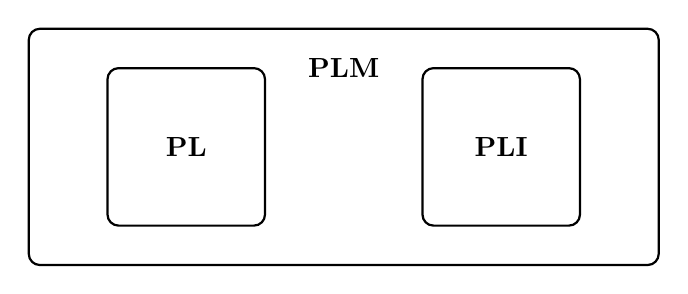
\begin{tikzpicture}
    
    \draw[thick, rounded corners] (-4, -1.5) rectangle (4, 1.5);
    
    \draw[thick, rounded corners] (-3, -1) rectangle (-1, 1);
    \node at (-2, 0) {\textbf{PL}};
    
    \draw[thick, rounded corners] (1, -1) rectangle (3, 1);
    \node at (2, 0) {\textbf{PLI}};
    
    \node at (0, 1) {\textbf{PLM}};
    
  \end{tikzpicture}
\end{center}
  
  


Un problema PL può sempre essere espresso nella seguente forma matriciale:
\[
  \max \{cx \mid Ax \leq b\}
\]
dove $ A \in \mathbb{R}^{m \times n} $ e $ b \in \mathbb{R}^m $. Grazie ad alcuni accorgimenti è possibile, inoltre, scrivere tutti i vincoli possibili di un problema di PL $\mathcal{P}$ in un'unico sistema di disequazioni lineari. Infatti:
\begin{itemize}
  \item Se \p è un problema di minimo, occorre considerare semplicemente la funzione $f (x) = (-c)x$
  \item Ogni vincolo $ax = b $diventa la coppia di vincoli $ax \leq b$ e $ax \geq b$
  \item Ogni vincolo $ax \geq b$ è equivalente a $(-a)x \leq (-b)$.
\end{itemize}

\ex{Pianificazione della Produzione}{
  \textbf{TESTO}

  La societ`a Pintel deve pianificare la produzione della sua fabbrica di micro-
processori. La Pintel possiede due diverse linee di prodotti: i processori Pin-
tium, pi`u potenti e destinati al mercato “server”, ed i Coloron, meno potenti
e destinati al mercato “consumer”. L’impianto `e in grado di realizzare 3.000
“wafer” alla settimana: su ogni wafer trovano posto o 500 Coloron oppure
300 Pintium. La resa di un wafer dipende anch’essa dal tipo di processore:
i Coloron, di minori dimensioni, hanno una resa media del 60\%, mentre i
Pintium, pi`u grandi e quindi maggiormente sottoposti a difetti, solamente
del 50\%. I processori Pintium si vendono a 500\$ al pezzo, mentre i Coloron
si vendono a 200\$ al pezzo. La divisione commerciale della Pintel ha anche
stabilito che la massima quantit`a di processori che possono essere messi sul
mercato ogni settimana senza causare un calo dei prezzi `e di 400.000 unit`a
per i Pintium e di 700.000 unit`a per i Coloron. Si vuole determinare le
quantit`a di ciascun tipo di processore da produrre settimanalmente in modo
da massimizzare il ricavo totale.

\textbf{SVOLGIMENTO}

  \begin{itemize}
    \item \underline{VARIABILI}

      Prendiamo le prime due variabili ovvie:
      \begin{align*}
        x_p = \text{"numero di pintium prodotti"}\\
        x_c = \text{"numero di coloron prodotti"}
      \end{align*}
      Notare che a differenza delle dispenze, $ x_p $ e $ x_c $ sono il numero di processori che \textit{proviamo} a produrre, senza tenere conto della resa del wafer.

      Usiamo anche due variabili che poi possiamo anche rimuovere:
      \begin{align*}
      w_p = \text{"numero wafer utilizzati per pintium"}\\
        w_c = \text{"numero wafer coloron"}
      \end{align*}
    \item \underline{VINCOLI}

      Mettiamo i vincoli di produzione settimanali:
      \begin{align*}
      0 \leq x_p 0.5 \leq 400000\\
        0 \leq x_c 0.6 \leq 700000
      \end{align*}

      Dobbiamo considerare anche il massimo numero di wafer, ipotizzo che un wafer puo' essere usato tutto solo per pintium o solo per coloron:
      \begin{align*}
        w_p + w_c \leq 3000
      \end{align*}

      Queste nuove variabili devono essere legate in qualche modo a quelle principali che usiamo nella FO:
      \begin{align*}
        300 w_p = x_p\\
        500 w_c = x_c
      \end{align*}

      Possiamo quindi tornare sul vincolo sul numero di wafer e sostituire $ w_p, w_c $ con $ x_p, x_c $ per riscrivere il vincolo relativo alle ultime due variabili, riducendo quindi le variabili utilizzate e semplificando il problema:

      \begin{align*}
      5 x_p + 3 x_c \leq 4500000
      \end{align*}

      L'insieme delle soluzioni ammissibili e' quindi:
      \[
        F = \{(x_p, x_c) | 0 \leq x_p 0.5 \leq 400000, 0 \leq x_c 0.6 \leq 700000, 5 x_p + 3 x_c \leq 4500000\}
      \]
    \item \underline{Funzione Obbiettivo}

      Vogliamo trovare $ max \{c(x_p, x_c) | (x_p, x_c) \in F \} $
      \[
        c(x_p, x_c) = 0.5 x_p \cdot 500 + 0.6 x_c \cdot 200
      \]

      Vediamo su un grafico l'area delle soluzioni ammissibili data da $ F $:
      \begin{center}
        \includegraphics[width=0.5\textwidth]{img/2025-03-03-12-33-31.png}
      \end{center}

      Un'importante proprieta' dei problemi lineari (reali) e' che la soluzione ottimale si trova sempre su uno dei "vertici" della figura descritta dalle soluzioni ammissibili (in questo caso quella ottimale e' (400000,100000) per $ (x_p/0.5, x_c/0.6) $).

      Grafico della funzione costo (rossa) con l'area delle soluzioni ammissibili (blu):
      \begin{center}
        \includegraphics[width=0.5\textwidth]{img/2025-03-03-12-50-44.png}
      \end{center}

      \textbf{OSSERVAZIONI}

      In realta', con la soluzione trovata il numero di wafer per tipo di chip non e' intero! In questo caso possiamo supporre che non sia troppo un problema, ma in altri casi puo' esserlo, quindi tocca studiare la \textit{programmazione lineare intera}.

 \end{itemize}

}

\subsection{Programmazione lineare intera}
Se nella $PL$ le variabili rappresentano quantità nella PLI le variabili possono essere
\begin{itemize}
  \item \textbf{Quantitative}: ovvero rappresentare quantità.
  \item \textbf{Logiche}: rappresentare valori booleani, ovvero scelte basate sulla possibilità di scegliere o meno una determinata opzione
\end{itemize}

Qui la definizione di variabile logica

\dfn{variabile logica}{
  Una \textbf{variabile} $x$ si definisce \textbf{logica} se:
  \[
    x \in \mathbb{N} (o \mathbb{Z}) \quad 0\leq x \quad x \leq 1
  \]
}

Un esempio tipico è rappresentato dalle variabili che associano una determinata risorsa a un compito specifico, oppure che determinano l'utilizzo di un particolare processo.

\begin{quote}
  Questo e' il bello dei problemi lineari

  \hfill -- Il Basta
\end{quote}

Un giga esempietto bellino è il problema dello zaino:
\ex{Problema dello zaino}{
  Il problema dello zaino è un esempio classico di problema di ottimizzazione combinatoria piuttosto complesso.

Sia dato un insieme E = {1, 2, . . . , n} di elementi, a ciascuno dei quali
sia assegnato un peso ai ed un costo ci, i = 1, . . . , n, interi e positivi: il
problema dello zaino (KP, da Knapsack Problem) consiste nel determinare
un sottoinsieme di elementi che abbia costo totale massimo ed il cui peso
totale non superi un prefissato intero b. 
  \vspace{1em}
  \textbf{Parametri:}
  \begin{align*}
    E &= \{1, \ldots, n\} \\
    a_i &= \text{peso dell'oggetto } i \\
    c_i &= \text{costo dell'oggetto } i \\
    b &= \text{peso massimo dello zaino}
  \end{align*}

  \vspace{1em}
  \textbf{Variabili:}

  Dobbiamo indicare usando le variabili quali elementi vogliamo includere nella soluzione e quali vogliamo scartare. Possiamo fare cio usando $ n $ variabili logiche:
  \begin{align*}
  x_i &=
  \begin{cases}
  1 & \text{se l'oggetto } i \text{ è nello zaino} \\
  0 & \text{altrimenti}
  \end{cases} \\
  x_i &\in \{0, 1\} \quad \forall i \in \{1, \ldots, n\}
  \end{align*}

  \vspace{1em}
  \textbf{Vincoli:}
  \[
    \sum_{i=1}^{n} x_i a_i \leq b
  \]

  \vspace{1em}
  \textbf{Funzione obiettivo:}
  \[
    \max \sum_{i=1}^{n} x_i c_i
  \]

}


\subsubsection{Relazioni logiche}

Avendo introdotto le variabili logiche, è opportuno chiedersi se sia possibile esprimere, mediante programmazione lineare (PL), le regole di inferenza logica per le relazioni che intercorrono tra di esse. Grazie all'uso di opportuni vincoli lineari, la risposta è affermativa:

\begin{itemize}
  \item \textbf{Negazione} \( (y = \neg x) \):
    \[
    x = 1 - y
    \]

  \item \textbf{Congiunzione} \( (z = x \land y) \):
    \[
    \begin{aligned}
      &z \leq x \\
      &z \leq y \\
      &z \geq x + y - 1
    \end{aligned}
    \]

  \item \textbf{Disgiunzione} \( (z = x \lor y) \):
    \[
    \begin{aligned}
      &z \geq x \\
      &z \geq y \\
      &z \leq x + y
    \end{aligned}
    \]

  \item \textbf{Implicazione} \( (z = x \implies y) \):
    \[
    \begin{aligned}
      &x + z \geq 1 \\
      &z \geq y \\
      &x + z \leq 1 + y
    \end{aligned}
    \]
\end{itemize}

È possibile, tuttavia, dimostrare che il problema di ottimizzazione lineare è, in generale, \textit{NP-hard}, dato che il problema di soddisfacibilità di una formula logica rientra nella classe NP-hard
\section{Template per risolvere problemi}

\subsection{Vincoli di assegnamento}
Un tipo di vincolo che la programmazione lineare intera (PLI) gestisce in modo molto efficace è rappresentato dai cosiddetti \textit{vincoli di assegnamento}. Questi vincoli sono utilizzati per modellare problemi che riguardano l'assegnazione di "oggetti a luoghi".

Si considerano:
\begin{itemize}
  \item Un insieme \( N = \{1, \ldots, n\} \) di \textbf{oggetti} (che possono rappresentare automezzi, persone, ecc.)
  \item Un insieme \( V = \{1, \ldots, m\} \) di \textbf{luoghi}
\end{itemize}

Per rappresentare le diverse condizioni di assegnazione degli oggetti ai luoghi, si introduce la variabile \( x_{ij} \in \{0, 1\} \) (dove \( 1 \leq i \leq n \) e \( 1 \leq j \leq m \)). Questa variabile indica se l'i-esimo oggetto è stato assegnato al j-esimo luogo (\( x_{ij} = 1 \)) o meno (\( x_{ij} = 0 \)), si può così procedere alla formale

\dfn{Vincoli di assegnamento}{
  Sia \( N = \{1, \ldots, n\} \) un insieme di oggetti e \( V = \{1, \ldots, m\} \) di luoghi, si definiscono \textbf{vincoli di assegnamento} quei vincoli che impongono che \textit{ogni oggetto sia assegnato a un solo luogo e ad ogni luogo è assegnato esattamente un oggetto}. Questi sono espressi mediante queste sommatorie:
  \[
    \sum_{j=1}^{m} x_{ij} = 1 \quad \forall i \in \{1, \ldots, n\} \quad \sum_{i=1}^{n} x_{ij} = 1 \quad \forall j \in \{1, \ldots, m\}
  \]

  Dove:
  \begin{itemize}
    \item \( x_{ij} \) è una variabile binaria che vale 1 se l'oggetto \( i \) è assegnato al luogo \( j \), e 0 altrimenti.
    \item La prima equazione assicura che ogni oggetto \( i \) sia assegnato esattamente a un luogo.
    \item La seconda equazione assicura che ogni luogo \( j \) riceva esattamente un oggetto.
  \end{itemize}
}

il luogo può anche essere visto come uno slot temporale, quindi imponiamo un certo pipeline


\subsubsection{Vincoli di semi-assegnamento}
I vincoli di semi-assegnamento sono una variante dei vincoli di assegnamento in cui non è necessario che ogni luogo riceva esattamente un oggetto, in particole si noti la seguente definizione

\dfn{Vincoli di semi-assegnamento}{
  Sia \( N = \{1, \ldots, n\} \) un insieme di oggetti e \( V = \{1, \ldots, m\} \) un insieme di luoghi. Si definiscono \textbf{vincoli di semi-assegnamento} quei vincoli che impongono che \textit{ogni oggetto sia assegnato ad al massimo un luogo}. Questi vincoli sono espressi mediante la seguente sommatoria:

  \[
  \sum_{j=1}^{m} x_{ij} \leq 1 \quad \forall i \in \{1, \ldots, n\}
  \]
  
  Dove \( x_{ij} \) è una variabile binaria che vale 1 se l'oggetto \( i \) è assegnato al luogo \( j \), e 0 altrimenti.
  

}

\ex{Problema del docente di informatica}{
  
\textbf{Testo}

Si hanno dei progetti ($t_1, t_2, \dots, t_n$), si hanno $m$ PC, dove ogni pc può compilare qualunque progetto in modalità sequenziale. Le prestazioni del PC sono identiche 

Vogliamo assegnare i progetti ai pc in modo da minimizzare il tempo complessivo parallelo di compilazione

\textbf{Svolgimento}

\textit{Variabili}:
\[
    \begin{aligned}
        x_{ij} &= \begin{cases}
            1 & \text{se il progetto $i$ è compilato al pc $j$} \\
            0 & \text{altrimenti}
        \end{cases}\\
        x_{ij}&\in \mathbb{N}, \quad \forall i\in \{1,\dots, n\}\,\forall j\in \{1,\dots, m\} \
    \end{aligned}
\]
\textit{Vincoli}:
\[
    \begin{aligned}
        \forall i\in\{1,\dots,n\}\quad \sum_{j=1}^{m}x_{ij} &= 1 \text{ (normale vincolo di semi-assegnamento!!)}\\
        \forall j\in\{1,\dots,m\}\quad y&\geq \sum^n_{i=1}x_{ij}t_i 
    \end{aligned}
\]
\textit{Funzione obbiettivo}:
\[
    \min (\underbrace{{\max_j \sum^n_{i=1}\underbrace{x_{ij}t_i}_{\text{tempo di compilazione del progetto $i$ al pc $j$}}}}_{\text{nonostante questa espressione matematica ha perfettamente senso, non è lineare!}})
\]

Funzione obbiettivo sbagliata! Pertanto prenderemo $y$ per "simulare" il massimo, di modo da rendere la funzione obbiettivo lineare:
\[
    \min y
\]
}

\subsection{Selezione di Sottoinsiemi}

Sia $ N = \{1,...,n\} $ un insieme finito di elementi e sia $ F = \{F_1,...,F_n\} $ una famiglia di sottoinsiemi (non necessariamente disgiunti) dove $F_i \subseteq N$ e sia $c_j$ un costo che associamo ad ogni $F_j$. Si vuole determinare qual'e' la scelta migliore di $ D\subseteq F $ di costo minimo fra tutti gli $F_j\in F$. Per formulare formalmente il problema, si può rappresentare l'appartenenza degli elementi di $ N $ in un sottoinsieme $ F_j $ come una matrice che ha un numero di $n$ righe (numero di elementi) e un numero $m$ di colonne (il numero di sottoinsieme). In dettaglio, sia $A=(a_{ij}\in\{0,1\}^{n\times m})$, dove
\[
  a_{ij} = \begin{cases}
    1 & \text{se } i \in F_j\\
    0 & \text{altrimenti}
  \end{cases}
\]

Il vettore delle variabili $ x $ assumerà la forma $ x = (x_1,...,x_m) $ dove
\[
  x_j = \begin{cases}
  1 & F_j \in D\\
  0 & \text{altrimenti}
  \end{cases}
\]
Definendo $D$ come $D = \{F_j \mid x_j = 1\}$

La funzione obbiettivo e' sempre:
\[
\sum_{j=1}^{n} x_j c_j
\]

I vincoli, invece, dipendono dal problema:
\begin{itemize}
\item \textbf{Problema di copertura}: ognuno degli elementi di $N$ sta in almeno uno degli elementi di $ D $:
    \[
      \sum_{j=1}^{m} a_{ij}x_j \geq 1 \quad \forall i \in [1,n]
    \]
   Ad esempio, i sottoinsiemi $ F $ di $ N $ possono essere dei curriculum dove c'è scritto quale dei linguaggi di programmazione $ l \in N $ conosce un candidato. Ogni candidato ha anche uno stipendio. Dobbiamo scegliere quali candidati assumere per coprire tutti i linguaggi in $ N $ minimizzando il costo
  \item \textbf{Partizione}: Ognuno degli elementi si $N$ sta in \textit{esattamente} uno degli elementi di $D$, ovvero $D$ deve essere una partizione di $ N $. Quindi:
    \[
    \sum_{j=1}^{m} a_{ij}x_j = 1 \quad \forall i \in [1,n]
    \]
    Ad esempio, $ N $ possono essere dei task da svolgere e gli iniemi di $ F $ sono offerte da fornitori rispetto alla risoluzione di alcuni dei task. Quindi gli inisiemi di $ D $ devono essere disgiunti perche' non vogliamo che due societa' risolvano lo stesso task. Tutto deve essere coperto una sola volta.

  \item \textbf{Riempimento}: si usa solo quando si vuole massimizzare il costo $c_j$. $ N $ non sono piu' incombenze o task, ma risorse da usare una volta per costruire un prodotto (elemento di $ F $). Al piu' perche' possiamo scartare qualche componente. Possiamo usare ogni elemento di $ N $ al massimo una volta. Quinidi:
  \[
    \sum^m_{j=1} a_{ij}x_j \leq 1 \quad \forall i\in [1,n]
  \]
\ex{Problema delle Commesse}{
\textbf{Testo}

Un'azienda deve decidere come impiegare i suoi $n$ dipendenti $1,\dots, n$.

L'azienda, nell'intervallo di tempo desiderato deve evadere $m$ commesse $1,\dots, m$

Ciascuna commessa $j$ deve essere svolta dal sottoinsieme $D_j\subseteq\{1,\dots, n\}$ dei dipendenti dall'azienda. 

Ogni commessa, se evasa darebbe luogo ad un ricavo pari a $r_j$ euro.

Ogni dipendente può lavorare ad una singola commessa nell'unità di tempo 

\textbf{Svolgimento}

Si consideri che questo è un Problema di selezione di sottoinsiemi, infatti:
$\quad N=\{1,\dots,n\}$ elementi/dipendenti

$F = \{F_1, \dots, F_m\} \quad \text{dove } F_j$ è la $j$-esima commessa che rappresentiamo con il sottoinsieme di dipendenti che la devono svolgere (quindi $ F_j = D_j $).

\[
    a_{ij}= \begin{cases}
        1 & \text{se } i\in F_j\\
        0 & \text{altrimenti}
    \end{cases}
\]

\textit{Variabili}:
\[
    \begin{aligned}
        x_j= \begin{cases}
            1 & \text{se la commessa $j$ è evasa}\\
            0 & \text{altrimenti}
        \end{cases}\\
        x_j\in\mathbb{N} \quad \red{y_j\in\mathbb{N}}
    \end{aligned}
\]

\textit{Vincoli}:
\[
    \begin{aligned}
        0\leq x_j\leq 1 \quad \forall j\in\{1,\dots,m\} \quad \red{0\leq y_j\leq 1}\\
        \forall i\in\{1,\dots,n\}\quad \sum^m_{j=1}a_{ij}x_j &\leq 1 \quad \red{y_j=1-x_j}
    \end{aligned}
\]
\textit{Funzione obbiettivo}:
\[
    \max \sum^m_{j=1}r_jx_j \red{-\sum^m_{j=1}y_ip_j}
\]

Nota: le scritte in rosso sono una possibile modifica all'esercizio dove per ogni commessa non fatta c'e' una penalita $ p_j $.
}

\end{itemize}
\subsection{Variabili a valori discreti}
Spesso, tuttavia, le variabili in gioco sono vincolate ad assumere un valore da un insieme che non è $\{0,1\}$ o un intervallo continuo (come $\mathbb{N}$). Ad esempio si può essere interessati a vincolare $x$ in un inseime finito di valori $Z = \{z_1,...,z_k\}$ dove i vari $z_i$ sono valori reali distinti 

In questi casi, si possono utilizzare $n$ variabili ausiliarie $y_1,...,y_k$ che rappresentano l'appartenenza di $z$ a $Z$. In particolare, si definiscono le variabili $y_i$ come segue:
\[
  y_i = \begin{cases}
    1 & \text{se } z = z_i\\
    0 & \text{altrimenti}
  \end{cases}
\]
E sono vincolate come segue:
\[
  \sum_{i=1}^{k} y_i = 1 \quad x=\sum^n_{i=1}z_i y_i
\]

\ex{Progetto di reti}{
  \textbf{TESTO}

Si vogliono collegare le reti fognarie di alcuni centri residenziali e industriali
ad un impianto di depurazione e smaltimento. Ogni centro produce una
quantit`a nota di rifiuti (liquidi), ed `e necessario dimensionare opportuna-
mente l’impianto di collegamento al depuratore in modo da consentirne il
trasporto. Si possono scegliere condotte di diversa portata e il costo di messa
in opera di una condotta sar`a una funzione della sua portata.
Si consideri ad esempio il grafo G = (N, A) di figura 1.3(a) dove i nodi da
1 a 4 rappresentano i centri ed il nodo 5 rappresenta il depuratore. Accanto
ad ogni nodo `e indicata la quantit`a di liquido da depurare per unit`a di tempo
prodotta dal centro ad esso corrispondente.
Ogni arco $ (i,j) \in A $ rappresenta un possibile collegamento; fra di essi
andranno scelti quelli che verranno effettivamente costruiti, e per ciascuno
dei collegamenti costruiti si dovr`a determinare la portata. Osserviamo che
i collegamenti hanno una direzione prefissata di percorrenza.
Una soluzione ammissibile `e data da un insieme di collegamenti che ga-
rantiscano il fluire dei liquidi da tutti i centri fino al depuratore. In figura
1.3(b) `e rappresentata una possibile soluzione.

\begin{center}
  \includegraphics[width=0.5\textwidth]{img/2025-03-03-13-45-07.png}
\end{center}

\textbf{SVOLGIMENTO}
TODO: svolgi
}

\subsection{Minima quantità positiva}

Quando una variabile $x$ rappresenta un certo livello di produzione, possibile che il valore della variabile sia 
\[
  x  \in \{0\} \cup [l,u]
\] 
Dove:
\begin{itemize}
  \item $ l $ e' il livello minimo di produzione
  \item $ u $ e' il livello massimo di produzione
  \item 0 è l'assenza di produzione
\end{itemize}
Per modellare correttamente tale situazione di introduce una variabile ausiliaria logica $y\in \{0,1\}$ che indica la presenza o l'assenza di produzione, cosicché i vincoli siano:
\[
  x \geq ly \quad x \leq uy
\]
Infatti se $y=0$ allora $x=0$ e se $y=1$ allora $x\in [l,u]$

\subsection{Funzione a carico fisso}
\dfn{Funzione a carico fisso}{
  Una funzione $f(x)$ è detta a carico fisso se:
  \begin{equation}
    f(x) = \begin{cases}
      b+cx & \text{se } 0<x \leq u\\
      0 & \text{se }x=0
    \end{cases}
  \end{equation}
  Dove $b>0$ e $u$ è un opportuno reale positivo
}
Si noti il seguente grafico rappresentativo:
TODO: inserire il grafico

Questo tipo di funzione è molto utile per modellare situazioni in cui si ha un costo di investimento fisso $b$ per l'attivazione di un servizio, e un costo variabile $c$ (coefficiente angolare) per l'unità di prodotto, mentre il costo è nullo se il servizio non è attivato ($x= 0 \implies f(x) = 0$)

Per rappresentare, analiticamente, questa funzione si introduce, al solito, una variabile ausiliaria logica $y\in \{0,1\}$ che indica l'attivazione del servizio, cosicché i vincoli siano:
\[
  0\leq x \quad x \leq uy 
\]

Adesso è possibile sostituire la funzione a carico fisso tramite una nuova funzione $g:\mathbb{R}^2\to\mathbb{R}$ definita come segue:
\[
  g(x,y) = b(y) + cx
\]

Si ha infatti che
\[
  g(0,0) = 0 \quad g(x,1) = b + cx
\]
\nt{
  Si noti che se $y=0$ allora, per i vincoli introdotti poc'hanzi, si ha che $x=0$ (anche se non vale viceversa). In altre parole i vincoli introdotti non eslcudono la possibilità che sia contemporaneamente $y=1$ e $x=0$, in questo caso avremo $g(0,1)\neq f(0)$ (nasty). Di conseguenza la funzione $g$ non rappresenta perfettamente ed in modo univoco la funzione $f(x)$, ma dato che l'obbiettivo è \textit{minimizzare} la funzione $f(x)$, la soluzione $(x,y) = (0,1)$ viene esclusa essendo $g(0,1) = b > g(0,0) = 0 = f(0)$
}

\ex{Ordinamento di valori su macchine}{
    TODO: aggiungere questo bellissimo esempip
}

\subsection{Rappresentazioni del valore assoluto}

\subsubsection{Vincoli di valore assoluto}
Si può avere a che fare con un \textbf{vincolo} a "valore assoluto" del tipo:
\[
  |g(x)| \leq b
\]

Dove $g(x)$ è una funzione dell'insieme di variabili $x$ e $b$ è un valore reale positivo, in questo caso tale vincolo è espresso come la congiunzione di due vincoli:
\[
  g(x)\leq b \quad -g(x)\leq b
\]
Dato che se $g(x)\leq b$ il vincolo $-g(x)\geq -b$ e viceversa. Inoltre, se $g(x)$ è una funzione lineare, allora tale vincolo può essere espresso come un vincolo lineare.

\subsubsection{Funzioni obbiettivo a valore assoluto}
Vediamo ora come trattare una funzione obiettivo espressa mediante un valore assoluto. Si consideri una funzione obiettivo $|f(x)|$ da dover \textit{massimizzare} con $x\in X$. È sufficiente risolvere i due diversi problemi:

\[
  \max \{f(x)\mid x \in X\} \quad \max \{-f(x)\mid x \in X\}
\]
E scegliere come soluzione quella che fornisce il valore più alto della funzione obbiettivo

\textit{Anal}olgalmente, per i problemi di minimizzazione

\subsection{Funzioni definite a tratti}
Una funzione che è possibile riscontrare nella vita reale è il caso delle funzioni lineare a tratti

Si consideri la seguente funzione 
\begin{equation}
  f(x) = \begin{cases}
    b_1 + c_1x & x \in [a_1, a_2]\\
    b_2+c_2x & x \in (a_2, a_3]
  \end{cases}
\end{equation}

Dove assumiamo 
\[
  b_2 + c_2a_2 \geq b_1 + c_1a_2
\]

Si noti il seguente grafico:

TODO: INSERIRE GRAFICO

Come per il carico fisso vengono introdotte due variabili logiche ausiliarie $ y_1, y_2 $ con seguente significato:
\begin{equation}
  y_1 = \begin{cases}
    1 & \text{se } x \in [a_1, a_2]\\
    0 & \text{altrimenti}
  \end{cases} \quad y_2 = \begin{cases}
    1 & \text{se } x \in (a_2, a_3]\\
    0 & \text{altrimenti}
  \end{cases}
\end{equation}
Dovendo $x$ appartenere ad uno ed uno solo degli intervalli, si ha il seguente vincolo
\[
  y_1 + y_2 = 1
\]


Inoltre introduciamo variabili quantitative ausiliarie che ci dicono lo spostamento rispetto a un estremo dell'intervallo a cui appartiene $x$:
\begin{equation}
  z_1 = \begin{cases}
    x - a_1 & \text{se } x \in [a_1, a_2]\\
    0 & \text{altrimenti}
  \end{cases} \quad z_2 = \begin{cases}
    x - a_2 & \text{se } x \in (a_2, a_3]\\
    0 & \text{altrimenti}
  \end{cases}
\end{equation}
Infatti se $x\in[a_1, a_2]$, il valore $z_1$ ($=x-a_1$) non è che la prozione di valore di $x$ che "supera" $a_1$, pertanto il suo valore è limitato dalle disuguaglianze $0\leq z_1 \leq a_2 - a_1$, si ha quindi che un'altro vincolo:
\[
  0\leq  (z_1 \leq a_2 - a_1 y_1)y_1
\]

Con $y_1$ variabile definita prima utile a controllare se effettivamente $x\in [a_1,a_2]$. Analogo è il caso di $z_2$, che ci conduce al seguente vincolo:
\[
  0\leq z_2 \leq (a_3 - a_2 )y_2
\]

Riassumendo tutti i vincoli ottenuti, si ha:
\begin{equation}
  \label{eq:vincoli_tratti}
  \begin{aligned}
    y_1,y_2 &\in \{0,1\}\\
    y_1 + y_2 &= 1\\
    0\leq z_1 &\leq (a_2 - a_1)y_1\\
    0\leq z_2 &\leq (a_3 - a_2)y_2
  \end{aligned}
\end{equation} 

\nt{
  Si noti che i vincoli \ref{eq:vincoli_tratti} impongono che solo una delle due variabili $z_1$ e $z_2$ possa avere valore non nullo
}

\subsubsection{Rappresentazione di $f$ con funzione mutlivariabile}
Poi il basta mi spiegherà la sequente quote 
\begin{quote}
  Non c'e' niente che ci da la funzione da ottimizzare, abbiamo solo delle definizioni che sono dei semplici commenti, i vincoli lineari sono solo gli ultimi, ma non bastano
  \hfill -- \faWhatsapp  
\end{quote}

Vabbuò, adesso è possibile sostuire alla funzione $f(x)$ la seguente funzione $g:\mathbb{R}^4\to \mathbb{R}$:
\[
  \begin{aligned}
    g(z_1, z_2, y_1,y_2 ) &= b_1y_1 + c_1(a_1y_1+z_1) + b_2y_2 + c_2(a_2y_2 + z_2) \\
    &= y_1(b_1+c_1a_1)+c_1z_1 + y_2(b_2+c_2a_2) + c_2z_2
  \end{aligned}
\]
Con le variabili soggette ai vincoli \ref{eq:vincoli_tratti}. In questo modo è stato possibile rappresentare la funzione $f(x)$ (non lineare) come una funzione lineare a variabili continue definita du un opportuno insieme.

Si ha che il valore di $ f $ e' rappresentato \textit{univocamente} dalla quadrupla $(z_1, z_2,y_1,y_2)$, eccetto nel punto di non continuita' $a_2$ che può essere espresso con le due seguenti quadruple:
\[
  (a_2 - a_1, 0, 1, 0) \quad (0, 0, 0, 1)
\] 

Dei quali solo \textbf{primo} è accettabile per i vincoli dati. Se, però, supponiamo il problema sia un problema di \textit{minimo}, possiamo considerare il prblema come benigno, dato che:
\[
  g(0,0,0,1) = b_2+c_2a_2 \geq b_1+c_1a_2 = g(a_2-a_1,0,1,0)
\]

